\documentclass{beamer}
\usepackage{etex}
\usepackage[utf8]{inputenc}
\usepackage{color,graphicx}
\usepackage{hyperref}
\usepackage[english]{babel}
\usepackage{fancyhdr}
\usepackage{amssymb}
\usepackage{amsmath}
%\usepackage[rflt]{floatflt} % die beiden gibts bei mir nicht. geht aber auch ohne?
%\usepackage{booktabs}       %     -- ben 2013/09/19
\usepackage{tabularx}
\usepackage{listings}
\usepackage{xcolor}
\usepackage{verbatim}
\usepackage{helvet}
\usepackage[normalem]{ulem}

\lstset{language=Java,basicstyle=\ttfamily,linewidth=\textwidth,breaklines=true,breakatwhitespace=true}
\lstset{captionpos=b}
\lstset{showstringspaces=false}

\definecolor{red}{rgb}{.6,.15,.15}
\definecolor{green}{rgb}{.1,.5,.1}

\setlength{\tabcolsep}{2pt}

\title{SL2: Die Simple Language mit Modulsystem}
\author{Benjamin Bisping, Rico Jasper,\\Sebastian Lohmeier und Friedrich Psiorz}
\date{Compilerbauprojekt SoSe 2013\\
Technische Universität Berlin\\
20.09.2013}

\usefonttheme{structurebold}

\begin{document}

\begin{frame}
\titlepage
\end{frame}

\begin{frame}
\tableofcontents
\end{frame}

\section{Einführung}

\begin{frame}
\frametitle{Einführung}
SL: typsicher und funktional im Browser (JavaScript)

\begin{center}
$\downarrow$
\end{center}

SL2: unabhängig kompilierbare Module

\begin{itemize}
\item Moduldefinition und -import (auch für das Prelude)
\item Export und einfache Qualifizierung von Funktionen und
    Datentypen
\item Einbindung von Funktionen und Datentypen aus JavaScript
\item Anpassungen der Syntax und Semantik
\item Fehlermeldungen verbessert
\item Compilierung ins Dateisystem
\item Bibliotheken, Beispielprogramme und Tests
\end{itemize}
\end{frame}

\begin{frame}
\frametitle{Altes Framework}

\begin{figure}
\center{%
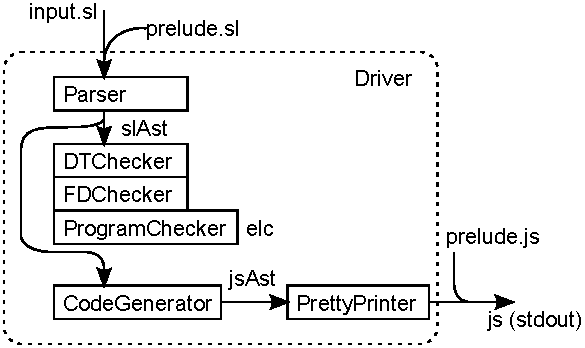
\includegraphics[width=1\linewidth]{programFlowOld}}
\end{figure}

\end{frame}

\begin{frame}
\frametitle{Neues Framework}

\begin{figure}
\center{%
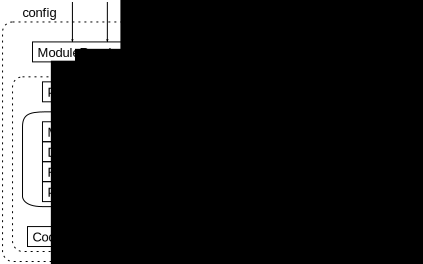
\includegraphics[width=1\linewidth]{programFlow}}
\end{figure}

\end{frame}

\section{Syntax und Parser}

\begin{frame}[containsverbatim=true]
\frametitle{Syntax -- Ausgangspunkt}
Typisch funktionale Syntax, ähnlich Haskell und Opal.

Besonderheiten:
\begin{itemize}
\item JavaScript-Blöcke:
  \begin{lstlisting}
  {| /* JS-Code */ |} : DOM Void
  \end{lstlisting}
 \item Fest eingebaute Funktionen und Operatoren:
   \begin{itemize}
     \item Standard-Operatoren für Ganzzahl-Arithmetik und
       Vergleiche
     \item \verb|+s|, \verb|+r|, \verb|*r|, etc. für
       Zeichenketten- und Gleitkomma-Operationen
     \item Unäres Minus auf Ganzzahlen (teilweise auch Gleitkomma) --
       Einziger unärer Operator, einzige überladene Funktion
     \item \texttt{\&} sowie \texttt{\&=} für Bind-Operation auf DOM-Monade
   \end{itemize}
 \item Eigene Funktionen und (binäre) Operatoren
   definierbar
\end{itemize}
\end{frame}

\begin{frame}
\frametitle{Syntax -- Zielsetzung}
\begin{itemize}
\item Unterscheidung zwischen eingebauten und 
  selbst definierten Operatoren aufheben
\item Modulsystem -- Syntax für Import, Export
  und Zugriff auf importierte Bezeichner
\item „Weniger Magie, mehr Bibliotheken“ -- Auch 
  Basis-Operatoren und -Funktionen sollten in 
  der Prelude und selbst geschriebenen Bibliotheken
  definiert werden können
\end{itemize}
\end{frame}

\begin{frame}[containsverbatim=true]
\frametitle{Anpassungen der Operatoren}
In SL2 werde alle Operatoren, abgesehen von der 
Präzedenz, gleich behandelt:
\begin{itemize}
\item Dürfen keine alphanumerischen Zeichen enthalten
\item Werden nicht überladen
\item Unäres Minus fällt weg, stattdessen Zahlen-Literale 
  mit negativem Vorzeichen
  \begin{itemize}
    \item Erlaubt: \verb|-2|, \verb|-.34e-13|
    \item Nicht erlaubt: \verb|-x|, \verb|- 2|, \verb|-(2)|
    \item Unintuitiv: \verb|x-2| ist Applikation \verb|x (-2)|
  \end{itemize}
\end{itemize}
$\Rightarrow$ Nicht schön, aber konsistenter als SL1
\end{frame}

\begin{frame}[containsverbatim=true]
\frametitle{Syntax für das Modulsystem}
Qualifizierter Import eines Moduls:
\begin{lstlisting}
IMPORT "path/to/module" AS MyModule
\end{lstlisting}

Zugriff auf importierte Bezeichner:
\begin{lstlisting}
MyModule.function
MyModule.Type
MyModule.Constructor
\end{lstlisting}

Export von Funktionen und Konstruktoren:
\begin{lstlisting}
PUBLIC DATA MyType = Cons1 | Cons2 | Cons3
PUBLIC FUN myFun : MyType -> Int
\end{lstlisting}
\end{frame}

\begin{frame}[containsverbatim=true]
\frametitle{Low-Level-Funktionalitäten}
Mit dem Keyword \verb|EXTERN| kann direkt auf die
JavaScript-Ebene zugegriffen werden.

\begin{itemize}
\item
Definition von Funktionen in JavaScript,
ohne DOM-Monade:
\begin{lstlisting}
DEF EXTERN function = {| js-code  |}
\end{lstlisting}
\item
Direktes Einfügen von JavaScript-Code in die Ausgabe:
\begin{lstlisting}
IMPORT EXTERN "path/to/js-file"
\end{lstlisting}
\item
Definition von Typen ohne Konstruktoren:
\begin{lstlisting}
DATA EXTERN TypeName
\end{lstlisting}
\end{itemize}
\end{frame}

\begin{frame}[containsverbatim=true]
\frametitle{Beispiel}
Auszug aus \emph{std/prelude}:
\begin{lstlisting}
-- Einfuegen der Datei _prelude.js
IMPORT EXTERN "std/_prelude"

-- Integer Datentyp ohne Konstruktoren
DATA EXTERN Int

-- Funktion _add definiert in _prelude.js
PUBLIC FUN + : Int -> Int -> Int
DEF EXTERN + = {| _add |}
\end{lstlisting}
\end{frame}

\begin{frame}
\frametitle{Parser}
Zwei Parser-Implementierungen:
\begin{itemize}
\item \emph{Parboiled-Parser} war Standard-Parser in SL1.
\item\emph{Combinator-Parser} hatte zu Beginn noch nicht
alle Features von SL1, ist jetzt unser Standard-Parser
wegen besserer Lokalisierung von Knoten im AST.
\end{itemize}
Beide Parser parsen SL2 korrekt.
\end{frame}

\section{Semantische Analyse}

\begin{frame}
\frametitle{Semantische Analyse}

\begin{enumerate}
\item Auflösung von Importen
\item Modulnormalisierung
\item Datentypen und Funktionen überprüfen
\item Type-Checking
\end{enumerate}

\end{frame}


\begin{frame}[containsverbatim=true]
\frametitle{Import-Überprüfung}

\begin{itemize}
\item Import-Anweisung: Paar aus Pfad und Bezeichner
	\begin{verbatim}
	IMPORT "path/to/module" AS MyModule
	\end{verbatim}
\item eineindeutige Modul-Bezeichner-Zuordnung
\item Annahme: genau ein Pfad identifiziert ein Modul
\item erlaubte Pfade:
	\begin{itemize}
	\item Kleinbuchstaben
	\item Zahlen
	\item Minus (-) und Unterstrich (\_)
	\item relative Pfade
	\end{itemize}
\end{itemize}

\end{frame}


\begin{frame}[containsverbatim=true]
\frametitle{Modulnormalisierung}

\begin{itemize}
\item keine modulübergreifende Modul-Bezeichner-Zuordnung
\item Normalisierung erforderlich
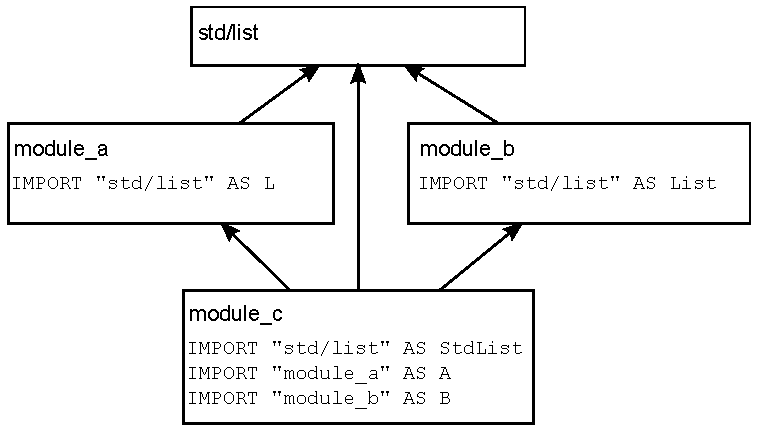
\includegraphics[width=1\linewidth]{depsModABC}
\item Substitution von \verb+L+ bzw. \verb+List+ durch \verb+StdList+
\end{itemize}


\end{frame}


\begin{frame}
\frametitle{Kontextprüfung}

\begin{itemize}
\item Berücksichtigung von importierten Datentypen und Funktionen
\item initialer Kontext um Modulkontext erweitert
\item Type-Checker weitestgehend unverändert
\end{itemize}

\end{frame}

\section{Codegenerierung und Signaturen}

\begin{frame}
\frametitle{Codegenerierung und Signaturen}
    - Rico - Signaturen
    - Sebastian - Codegenerierung
\end{frame}


\begin{frame}
\frametitle{Modulsignatur}

\begin{itemize}
\item Signatur für semantische Analyse erforderlich
\item Inhalt:
	\begin{itemize}
	\item Importliste
	\item Datendefinitionen
	\item Funktionssignaturen
	\end{itemize}
\item Mögliche Signaturformate:
	\begin{itemize}
	\item native Serialisierung
	\item SL
	\item JSON
	\end{itemize}
\end{itemize}

\end{frame}


\begin{frame}[containsverbatim=true]
\frametitle{Modulsignatur -- JSON}

\begin{verbatim}
IMPORT "some/module" AS M
\end{verbatim}

JSON:

\begin{lstlisting}
"imports" : [
  {
    "name" : "M",
    "path" : "some\/module"
  }
]
\end{lstlisting}


\end{frame}

\section{Fehlermeldungen}

\begin{frame}
\frametitle{Fehlermeldungen -- Ausgangspunkt}
Die bisherige Fehlerbehandlung in SL war unzureichend
\begin{itemize}
\item Parser parst nur bis zum ersten Syntaxfehler, gibt aber bis
  dahin gültige Teile des Programms einfach weiter
\item Statt Fehlermeldungen werden Scala-Objekte ausgegeben
\item Teilweise unbehandelte Exceptions; der Compiler beendet sich
  mit Stacktrace
\end{itemize}
$\Rightarrow$ Absolut unzureichend für jedes Projekt, das mehr als 
ein paar Zeilen Code umfasst.
\end{frame}

\begin{frame}[containsverbatim=true]
\frametitle{Fehlermeldungen -- Format}
\begin{lstlisting}
/path/to/file.sl:5:1-23: Use of undefined type(s) in `Foo': `Foo.Bar'
\end{lstlisting}
Das allgemeine Format ist folgendes:
\begin{center}
\emph{Dateiname} : \emph{Zeile(n)} [: \emph{Spalte(n)}] : \emph{Fehlermeldung}
\end{center}
Lokalisierung mit Zeilen- und Spaltennummer nur mit Combinator-Parser
\end{frame}

\begin{frame}
\frametitle{Fehlerarten}
\begin{itemize}
\item Syntaktische Fehler
  \begin{itemize}
  \item Häufige Fehler haben eigene Produktionen im Parser
  \item Teilweise nur kryptische Fehlermeldungen der Parsec-Bibliothek
  \item Abbruch nach erstem syntaktischen Fehler
  \end{itemize}
\item Semantische Fehler
  \begin{itemize}
  \item Typfehler werden erkannt, Ort teils unintuitiv
  \item Doppelte Deklarationen, fehlende Definitionen, falsche Aritäten, etc.
    werden mit Ort(en) zurückgegeben
  \end{itemize}
\item Importfehler
  \begin{itemize}
  \item Moduldateien nicht vorhanden: Ort des Import-Statements
    sowie Suchpfad für Datei werden ausgegeben
  \item Zyklische Importe, Qualifizierter Import der Prelude
  \end{itemize}
\item Laufzeitfehler werden vom JavaScript-Interpreter behandelt
\end{itemize}
\end{frame}

\section{Prelude und Bibliotheken}

\begin{frame}
\frametitle{Prelude und Bibliotheken}
- Ben
\end{frame}
\section{Beispielprogramme und Tests}

\begin{frame}
\frametitle{Beispielprogramme}

\begin{figure}
\center{%
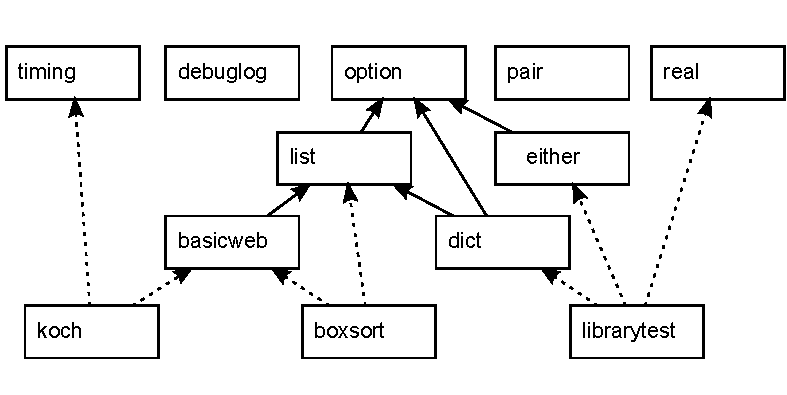
\includegraphics[width=1\linewidth]{depsSamples}}
\end{figure}
\end{frame}
\section{Fazit}

\begin{frame}
\frametitle{Fazit I}
\begin{itemize}
\item Modulare typsichere Webanwendungen im Browser und node.js möglich
\item Modulimporte, qualifizierte Bezeichner, Exporte
\item Fehlermeldungen verbessert
\item Prelude in Module überführt
\item initiale Standard-Bibliothek erstellt
\end{itemize}

$\rightarrow$ Pflichtenheft erfüllt
\end{frame}

\begin{frame}
\frametitle{Fazit II}
Mögliche Erweiterungen

\begin{itemize}
\item Flexiblerer Import
\item Statische zyklische Abhängigkeiten
\item Konfiguration der Codegenerierung für require.js
\item Verbesserte Typchecker-Fehlermeldungen
\item Erweiterte Bibliotheken
\end{itemize}
\end{frame}

%\section{Beamer-Beispiele}

\begin{frame}
\frametitle{Itemize und enumerate}
bullet points: itemize, Nummerierung: enumerate
\begin{itemize}
\item \textbf{EMMA} and \emph{motor modules}
\item Spreading activation with :bll 0.3 :mas 3 :rt 0 :ga 1
    :retrieval-activation 4 :visual-activation 2 :imaginal-activation 8
\item New TWM nodes created in imaginal buffer to keep parsing state
    and context in goal buffer
\item Word frequencies from dlexdb.de for base levels and EMMA
\end{itemize}
\end{frame}

\begin{frame}
\frametitle{Eine Tabelle}
\begin{table}[h]
\begin{center}
\begin{tabularx}{9cm}{Xll}
\toprule
Condition (2 items, 6 subjects) & DA & IA \\\midrule
Experiment (unreliable) & 3824ms & 3946ms \\
Model 1 & 3242ms & 3323ms \\
Model 2 & 3527ms & 3293ms \\
\bottomrule%
\end{tabularx}%
\end{center}%
\end{table}
\end{frame}

\begin{frame}[containsverbatim=true]
\frametitle{Quellcode anzeigen}
[containsverbatim=true] nach frame-Beginn nicht vergessen

\vskip 20pt

\begin{lstlisting}
for c in range(k):
   Mus[:,c]=X.T[np.where(rPrime==c)].T.mean(1)
\end{lstlisting}
\center{vs.}
\begin{lstlisting}
for i in range(k):
   mu[:,i] = np.mean(X[:,raux==i],axis=1)
\end{lstlisting}
\end{frame}

\begin{frame}[containsverbatim=true]
\frametitle{Grafiken einbinden}
Zur Skalierung einfach den Faktor ohne Multiplikationszeichen vor die
Breitenangabe schreiben.
\begin{figure}
\center{%
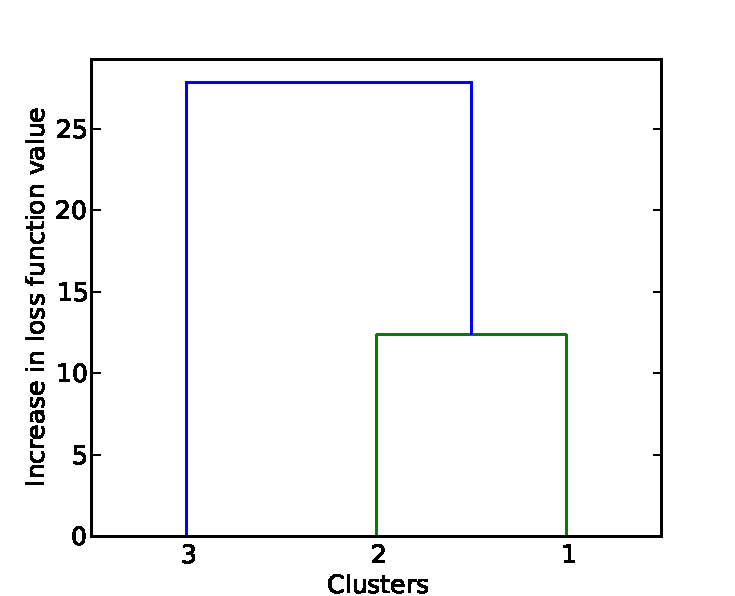
\includegraphics[width=.75\linewidth]{fig3}}
\end{figure}
\end{frame}

\end{document}